\chapter{Following Behaviours}
\label{chap:following}

In this chapter, we describe the design, implementation and testing of a mobile robot with following behaviours.
The mobile robot follows a designated person, while keeping a safe distance.
When the designate person is not on the scene, the robot should wander around to look for the person.

\section{Assumptions}

Several assumptions are made in our design of following behaviours.

\begin{enumerate}
    \item There is no obstacle between the person and the robot.
    \item When more than one person are on the scene, the robot is given instruction on which person to follow. That is, a person is designated to be followed.
    \item The designated person is dressed differently to other persons on the scene such that the robot can tell the difference.
\end{enumerate}

\section{System Design}

\subsection{Flow Chart}

A flow chart of the mobile robot is shown in Figure \ref{fig:following}.
When the robot starts and receives the first image from the camera, it locates all persons on the image using an object detection model \citep{howard2017mobilenets,liu2016ssd}.
If no person is found from the camera image, the robot activates "Wander Behaviour."
If one or more persons are located, for each person located, a bounding box and a confidence score are given by the model.

Each bounding box is resized and compared against the target image for a similarity score using the euclidean distance.
The person with the highest similarity score is selected.
During the comparing stage, the user may also change the target image to any bounding box of located person.
By default, the target image is a blank image.

If the highest similarity score is lower than $0.7$, "Wandering Behaviour" is activated.
Otherwise, both "Collision Avoidance Behaviour" and "Person Following Behaviour" are activated. However, the output action from "Collision Avoidance Behaviour" has higher priority than "Person Following Behaviour".

Once the robot finishes the action and receives a new update from the camera, it will repeat from locating all persons on the scene again.

\begin{figure}
\centering
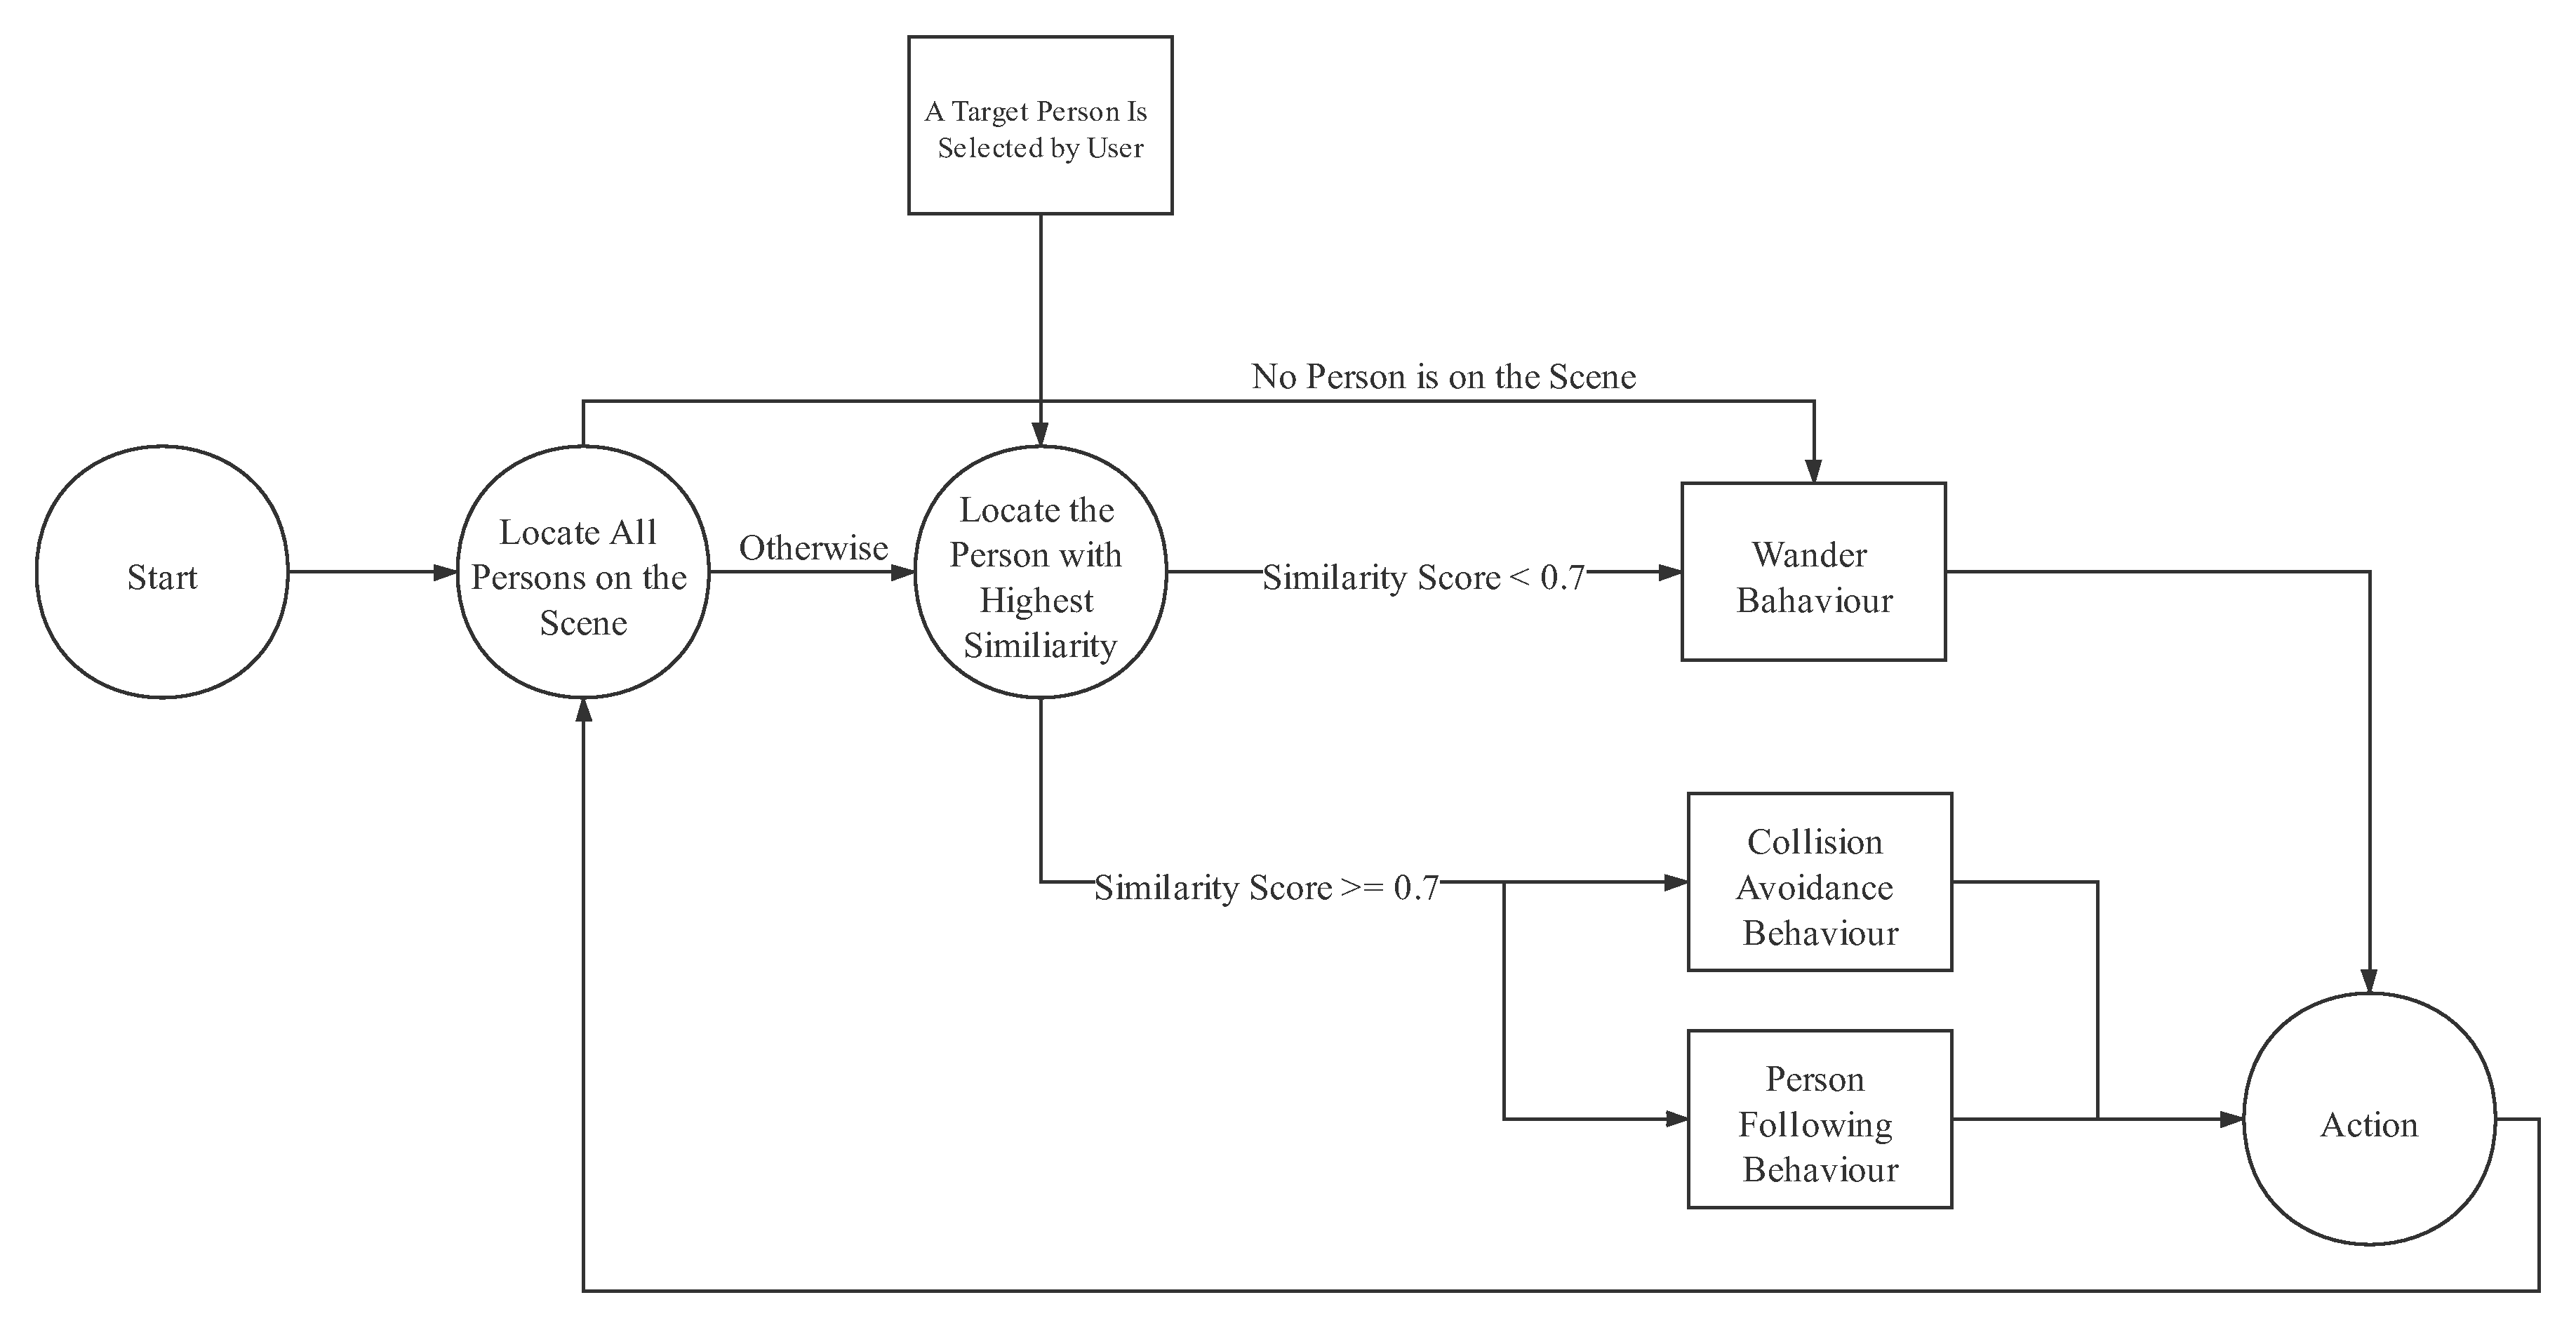
\includegraphics{following}
\caption{Flow Chart of the Mobile Robot with Following Behaviours.}
\label{fig:following}
\end{figure}

\subsection{Wandering}
Our initial design of Wandering behaviour is to keep moving forward and turn left when an obstacle is found in front of the robot.
However, we observe that such behaviour leads to frequent dead ends and bumping due to the size of the robot and the complexity of our environment.
The initial Wandering Behaviour is replaced with self-rotating as shown in Figure \ref{fig:wander}.
That way, the robot will keep rotating in the same direction until a person is located.
It will not move into the dead end or bump into the obstacle.

\begin{figure}
\centering
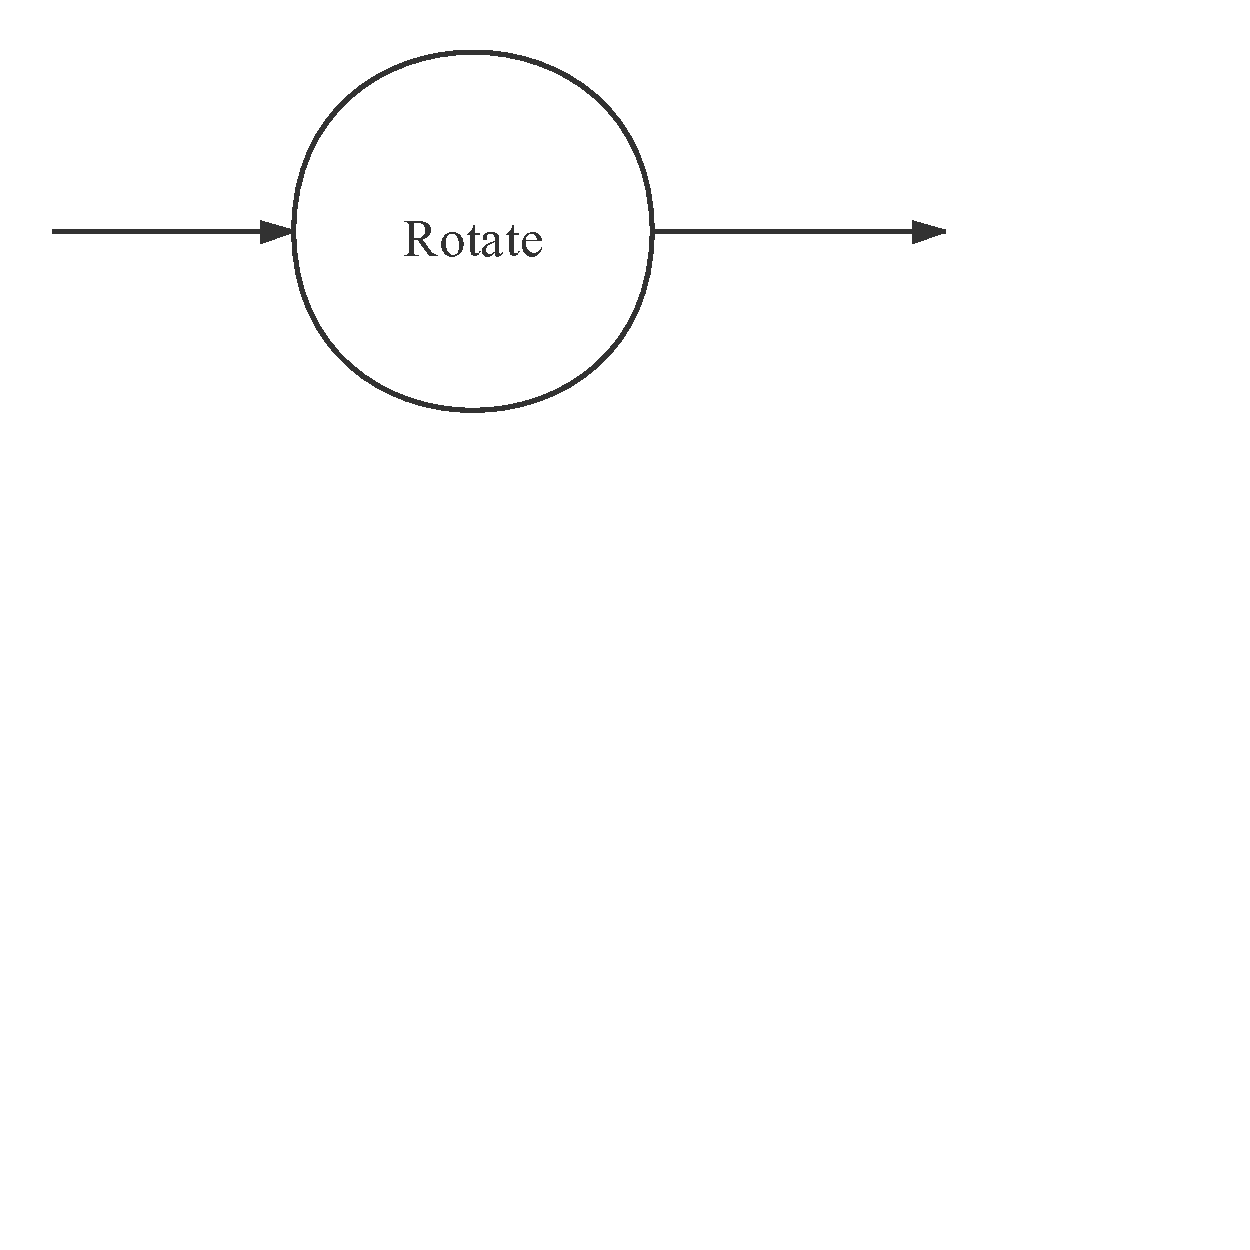
\includegraphics[width=0.5\textwidth]{wander}
\caption{Wandering Behaviour of the Mobile Robot.}
\label{fig:wander}
\end{figure}



\subsection{Collision Avoidance}
Collision Avoidance Behaviour prevents robot from bumping into the designated person and always has higher priority than Person Following Behaviour.
Figure \ref{fig:collision} describes the behaviour in details. The distance between the robot and the designated person is computed using the camera's depth information.
If the distance is smaller than $300$ mm, the robot moves backward to avoid bumping into the person.
If the distance is equal or larger than $300$ mm and smaller than $600$ mm, the robot stops moving.
Therefore, the robot always keeps a safe distance between $300$ and $600$ mm from the person when it stops moving.

\begin{figure}
\centering
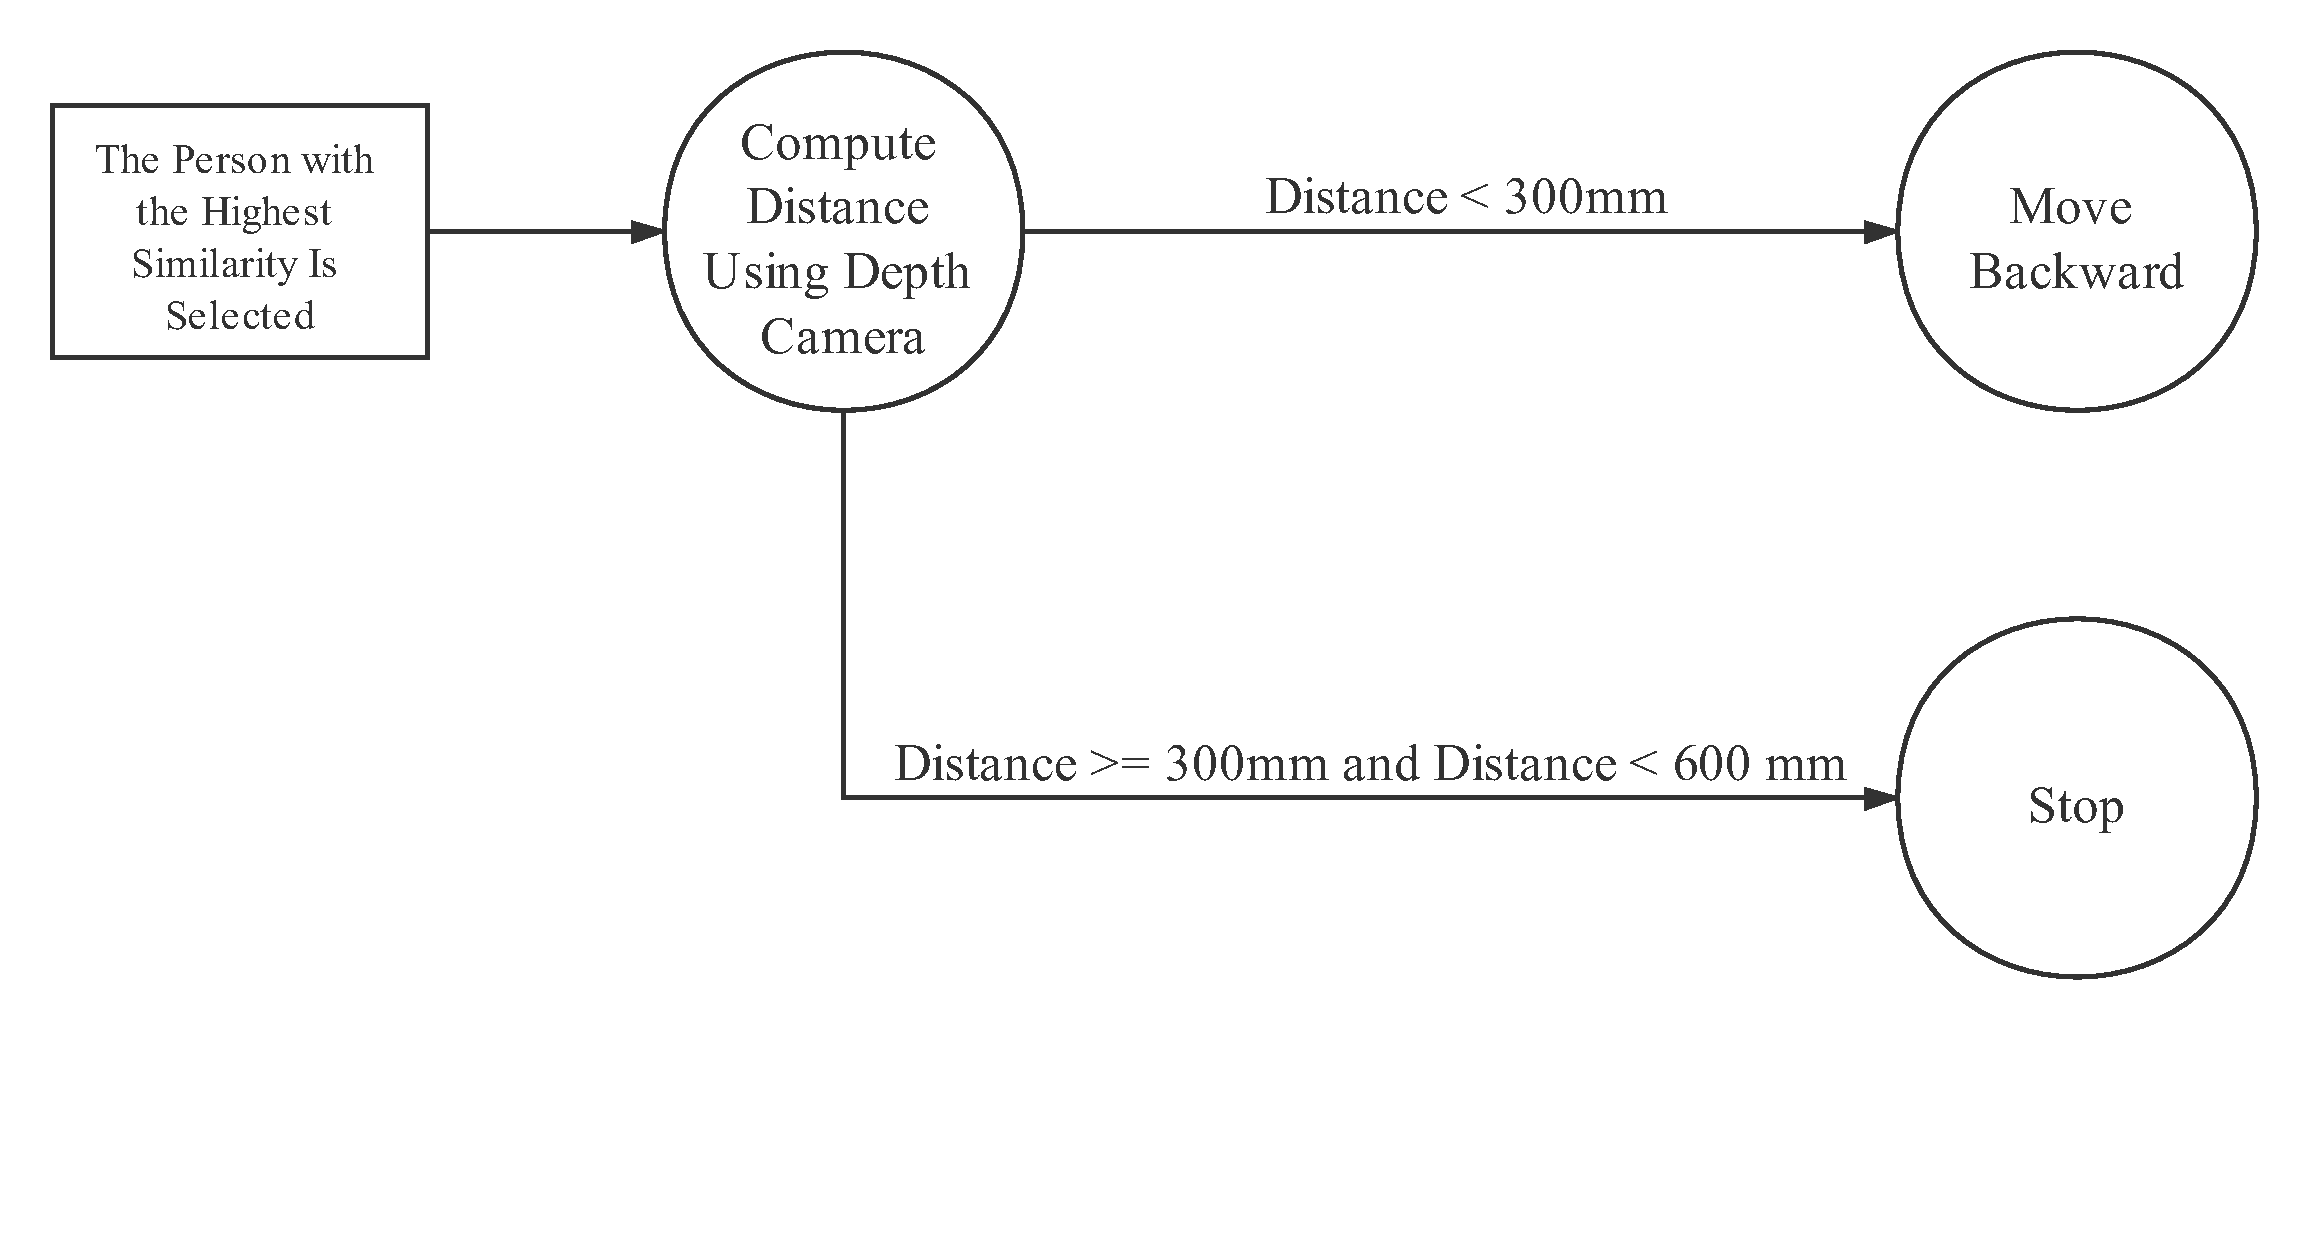
\includegraphics[width=\textwidth]{collision}
\caption{Collision Avoidance Behaviour of the Mobile Robot.}
\label{fig:collision}
\end{figure}

\subsection{Person Following}
Person Following Behaviour keeps tracking the designated person and moving the robot to the person.
Figure \ref{fig:person} describes the behaviour in details.
The target image is first replaced with the new bounding box if the similarity between them is larger then $0.9$.
This action keeps the robot updated with the information of the target. It prevents the robot from decreasing similarity score over time and losing the target in the end.

The center of the bounding box in x-axis is later computed to determine whether the person is on the left, center or right.
If the person is on the left side, the robot rotates to the left and vice versa.
If the person is in the center area, the robot moves forward.


\begin{figure}
\centering
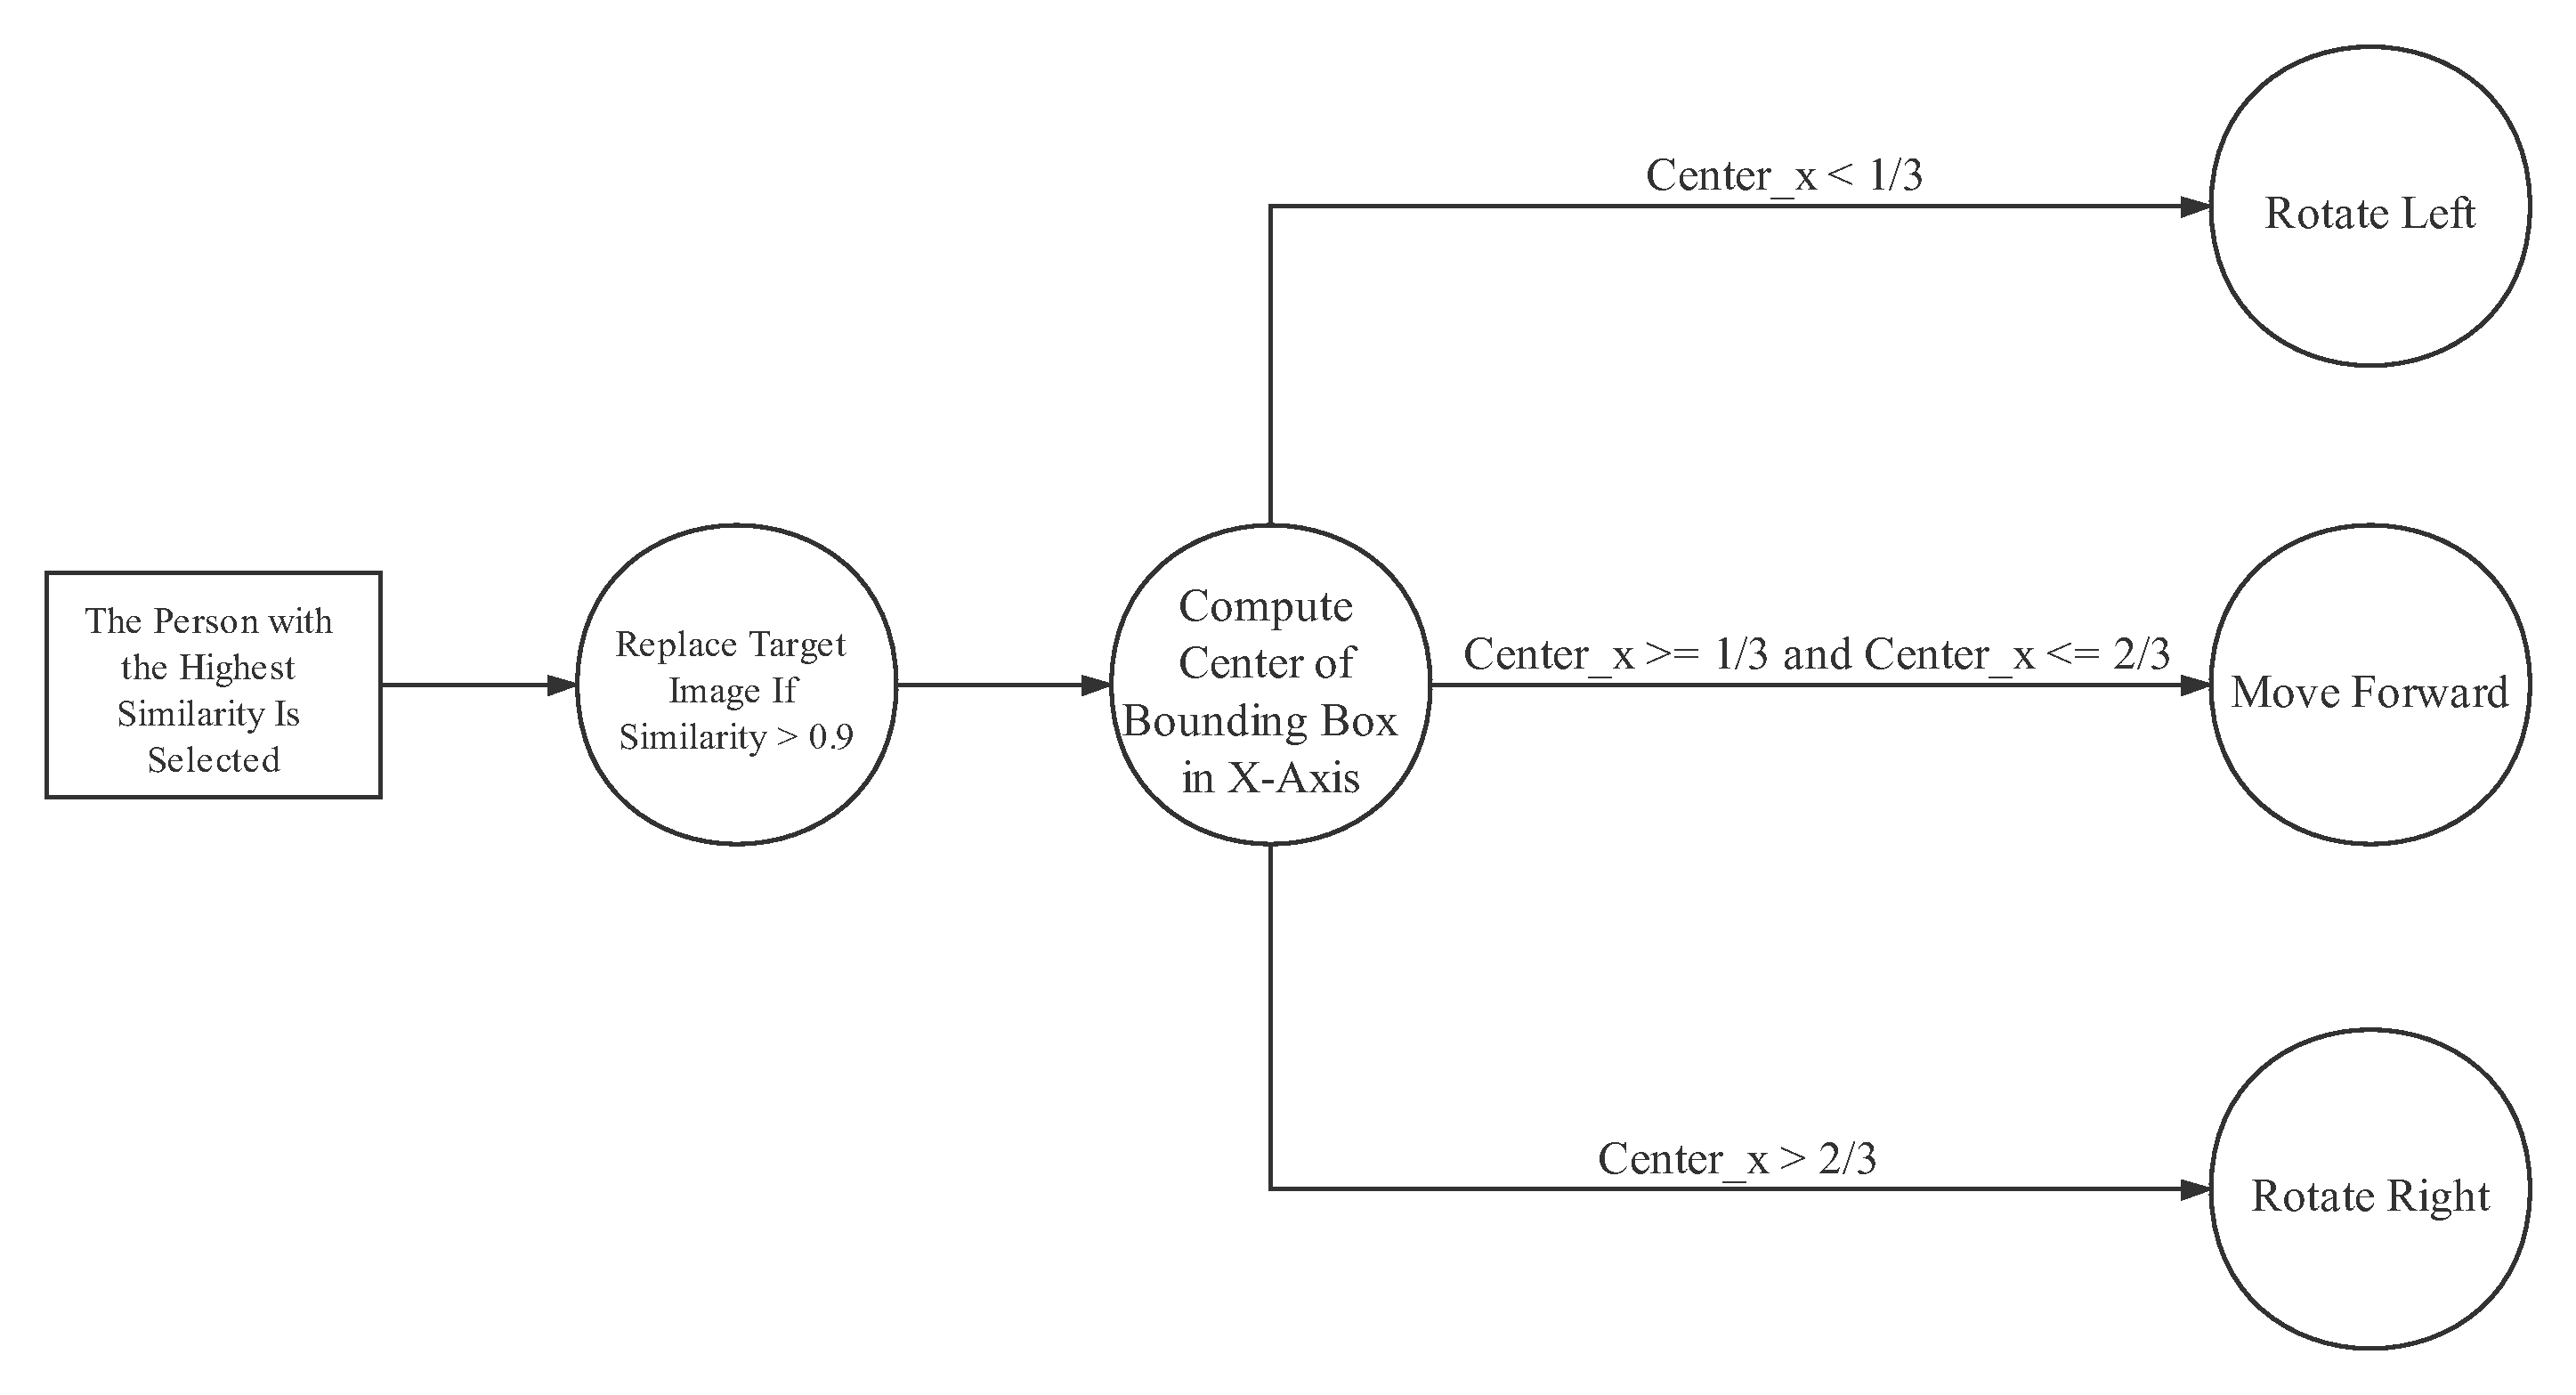
\includegraphics[width=\textwidth]{person}
\caption{Person Following Behaviour of the Mobile Robot.}
\label{fig:person}
\end{figure}

\section{Implementation}
The following behaviours are implemented in Python Programming Language and Jupyter Notebook environment.
The implementation uses the source code from Tutorial 5 as the framework and improves upon that.
Several important adjustments are made and described as follows.

\subsection{Computing Similarity Scores}
After all persons on the scene are located using a object detection model, a similarity score between bounding box of each person (variable named \texttt{obj}) and the target image (variable named \texttt{target}) is computed.
Both \texttt{obj} and \texttt{target} are resized to a resolution of 300-by-300 using \texttt{cv2.resize} function.
Both \texttt{obj} and \texttt{target} are converted to HSV color space using \texttt{cv2.cvtColor} function and later normalised through being divided by $255$.
The similarity score between \texttt{obj} and \texttt{target} is defined $1 - distance_{euclidean}(obj, target)$.

\subsection{Computing Distance}
In Collision Avoidance Behaviour, the distance between the designated person and the robot is computed.
Applying the bounding box of the person to the depth image, a matrix of depths inside the bounding area is retrieved.
The distance between the person and the robot is simply the minimum non-zero value in the matrix.

\section{Test \& Analysis}
Two testing scenarios are performed and analyzed in this section.

\subsection{Single Person Following}
In this scenario, only one person is presented in the environment.
The robot is expected to follow the person around the room.

Figure \ref{fig:follow-test} shows an video capture of our testing scenario.
As the person walks around in the room, the robot keeps following in a safe distance and never loses track of the person.

\begin{figure}
\centering
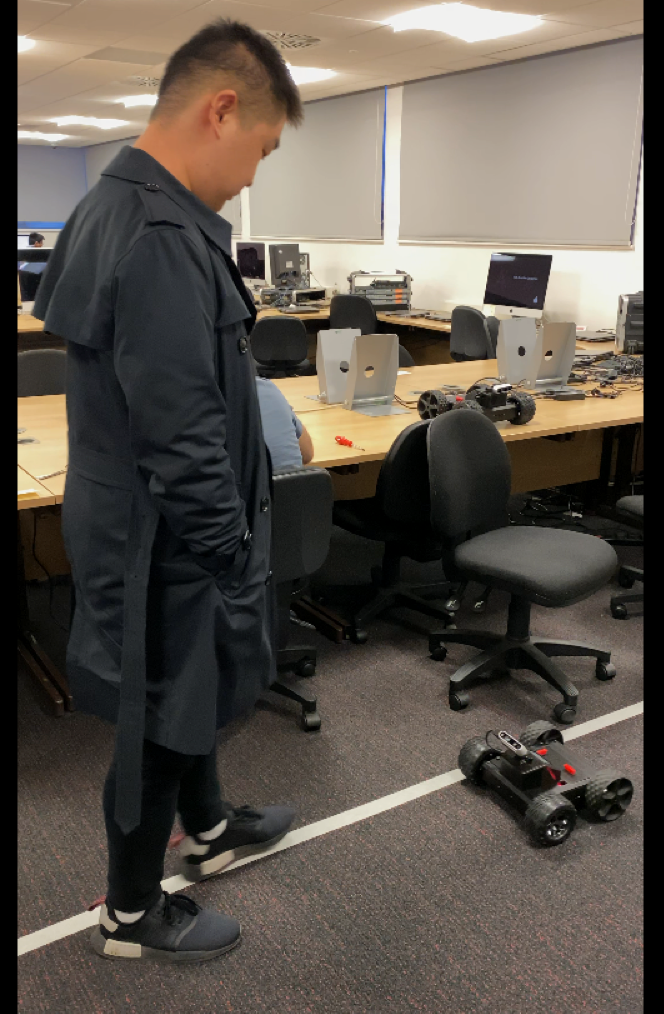
\includegraphics[width=0.8\textwidth]{follow-test}
\caption{Testing of Single Person Following.}
\label{fig:follow-test}
\end{figure}

\subsection{Single Person Following under Attempted Hijacking}
In this scenario, two persons are presented in the environment. One person is chosen as the designated person to follow.
The other person makes several attempts to hijack the robot by stepping in front of the designated person and then walking away.
The robot is expected to always follow the designated person and not follow the other person.

\begin{figure}
\centering
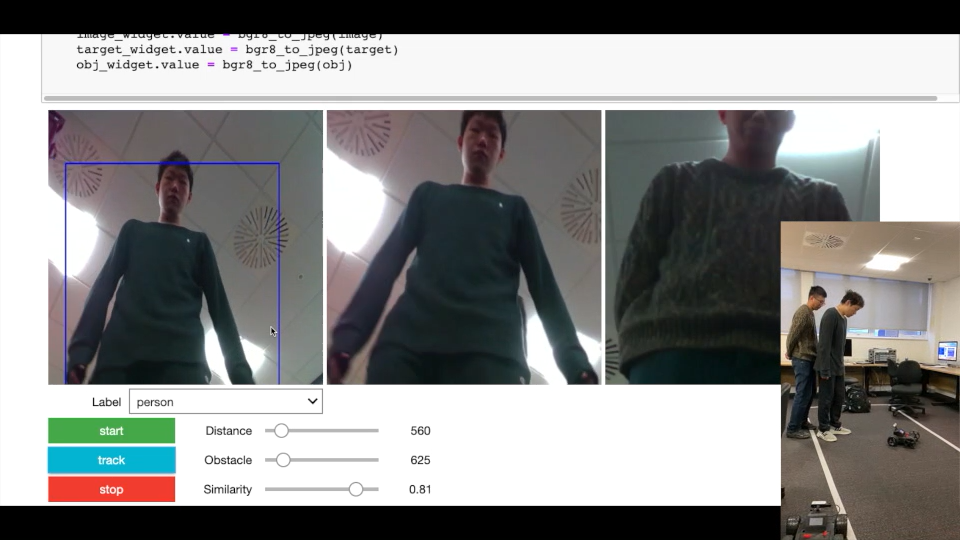
\includegraphics[width=0.8\textwidth]{follow-test-hijack}
\caption{Testing of Single Person Following under Attempted Hijacking.}
\label{fig:follow-test-hijack}
\end{figure}

Figure \ref{fig:follow-test-hijack} shows an video capture of our testing scenario.
The camera image is shown on the left, the bounding box the person in the center and the target image on the right.
The robot distinguishes between two persons by computing the similarity score between the bounding box and the target image.

As the designated person walks around in the room, the robot keeps following in a safe distance and never loses track of the person.
The other person makes several attempts to hijack the robot. However, the robot distinguishes between the two persons and does not follow the other person.

